\documentclass[12pt, letterpaper]{article}

% --- Packages ---
\usepackage{geometry}
 \geometry{margin=1in}
\usepackage{graphicx}
\usepackage{amsmath, amssymb}
\usepackage{booktabs}
\usepackage{hyperref}
\usepackage{cite}
\usepackage{setspace}
\onehalfspacing
\usepackage{fontspec}
\usepackage{polyglossia}
\usepackage{float}
\usepackage{svg}
\usepackage{enumitem}
\setmainlanguage{vietnamese}

\usepackage{listings}
\usepackage{xcolor}

\lstset{
    language=Python,
    basicstyle=\ttfamily\small,
    keywordstyle=\color{blue},
    stringstyle=\color{red},
    commentstyle=\color{green!60!black},
    breaklines=true,
    frame=single, % Tạo khung xung quanh code
    backgroundcolor=\color{gray!5}
}

\renewcommand{\lstlistingname}{Mã nguồn}

% --- Metadata ---
\title{Thiết kế PID cho hệ thống điều khiển nhiệt độ cho phản ứng hóa học}
\author{Đỗ Hoàng Gia Bảo - 23020783 \\ \small Khoa Điện tử - Viễn Thông}
\date{\today}

\begin{document}

\maketitle

\begin{abstract}
Báo cáo sẽ trình bày các bước thiết kế và lập trình bộ điều khiển PID cho hệ thống điều khiển nhiệt độ trong phản ứng hóa học. Chương trình được viết bằng Python sử dụng thư viện Tkinter để mô phỏng quá trình điều khiển và hiển thị kết quả. 
\end{abstract}
% --- Front Matter (Roman Numerals) ---
\newpage
\tableofcontents

% --- Main Content (Arabic Numerals) ---
\newpage
\pagenumbering{arabic}
\setcounter{page}{3} % This automatically resets the counter to 1

\section{Yêu cầu đề bài}
Một hệ thống điều khiển nhiệt độ cho một quá trình hóa học được thể hiện trong Hình dưới đây. Hệ thống chưa được bù đang
hoạt động với thời gian tăng xấp xỉ bằng một hệ thống bậc hai
với thời gian đạt đỉnh là $T_p = 16 \text{ giây}$ và độ Overshoot $\%OS = 5\%$.
Thiết kế bộ điều khiển PID sao cho hệ thống được bù sẽ có
thời gian tăng xấp xỉ tương đương với một hệ thống bậc hai
với thời gian đạt đỉnh là $T_p = 8 \text{ giây}$ và độ Overshoot $\%OS = 5\%$, và sai số trạng thái ổn định bằng không đối với tín hiệu đầu vào dạng bước.
\begin{figure}[H]
    \centering
    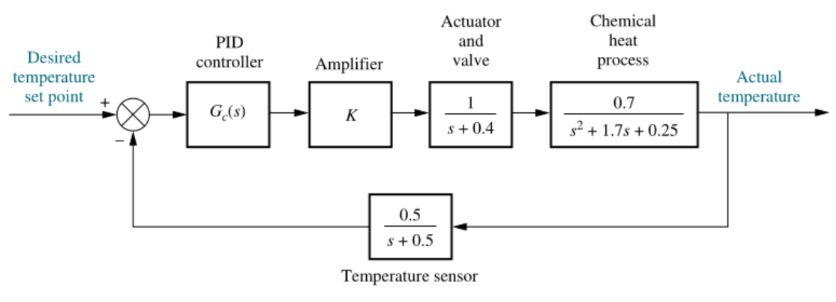
\includegraphics[width=0.9\textwidth]{Images/System.jpg}
    \label{fig:system}
\end{figure}

\section{Thiết kế  bộ điều khiển PID}
\subsection{Phân tích hệ thống khi chưa sử dụng bộ điều khiển PID}
Khi hệ thống chưa bù, hệ thống đang hoạt động với các thông số tương đương với hệ bậc hai là:
\begin{itemize}
    \item Peak Time $T_p = 16$
    \item Overshoot $\%OS = 5\%$
\end{itemize}
Qua các hệ số trên, ta có thể tìm được các cặp cực hiện tại của hệ thống thông qua các công thức cho hệ thống bậc hai.
\begin{enumerate}
    \item Hệ số suy giảm ($\zeta$)
    $$\zeta = \frac{-\ln(\%OS)}{\sqrt{\pi^2 + \ln^2(\%OS)}} = \frac{-\ln(0.05)}{\sqrt{\pi^2 + \ln^2(0.05)}} \approx 0.69$$

    \item Tần số tự nhiên ($\omega_n$)
    $$\omega_{n1} = \frac{\pi}{T_{p1}\sqrt{1 - \zeta^2}} = \frac{\pi}{16\sqrt{1 - 0.69^2}} \approx 0.272\text{ rad/s}$$

    \item Vị trí cực chưa bù ($s_{1, 2}$)
    $$s_{1,2} = -\zeta\omega_{n1} \pm j\omega_{n1}\sqrt{1-\zeta^2} = -0.69 \cdot 0.272 \pm j0.272\sqrt{1-0.69^2} \approx -0.187 \pm j0.196$$
\end{enumerate}
Từ các vị trí cực trên, ta có thể xác định hệ số khuếch đại $K$ khi hệ thống chưa bù sử dụng quỹ tích nghiệm (root locus).
\begin{enumerate}
    \item Xác định hệ thống vòng hở của hệ thống chưa bù
    $$G_{open}(s) = G_p(s) \cdot H(s) = K \cdot \frac{1}{s + 0.4} \cdot \frac{0.7}{s^2+1.7s+0.25} \cdot \frac{0.5}{s+0.5}$$
    $$G_{open}(s) = \frac{0.35K}{(s + 0.4)(s + 0.5)(s + 0.161)(s + 1.539)}$$
    \item Vẽ đường quỹ tích nghiệm dựa trên điểm không và điểm cực của hệ thống vòng hở.
    \begin{figure}[H]
        \centering
        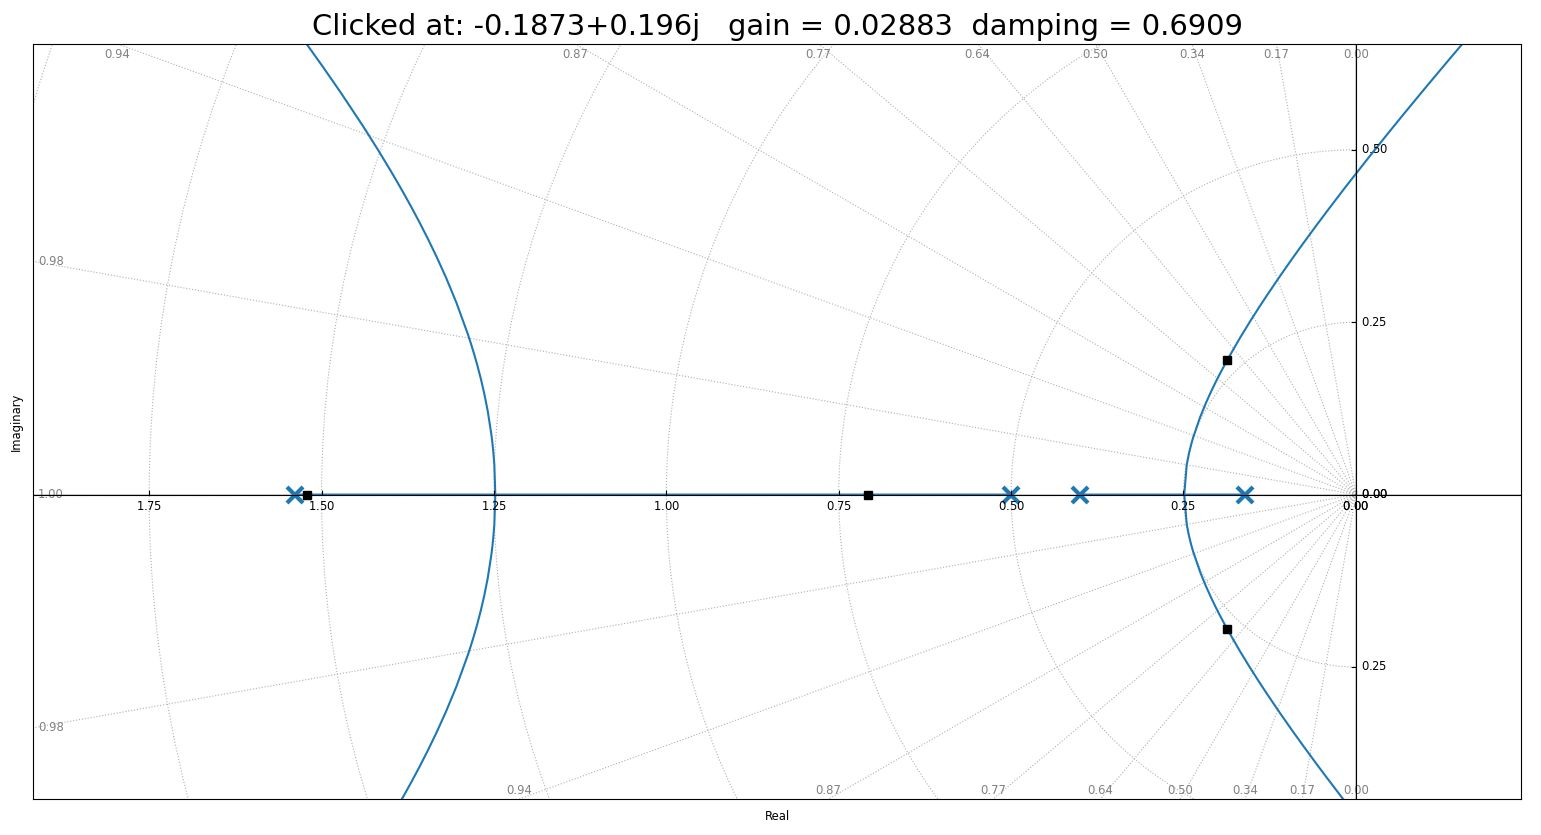
\includegraphics[width=0.9\textwidth]{Images/uncompensated_root_locus.jpg}
        \caption{Quỹ tích nghiệm của hệ thống khi chưa bù}
    \end{figure}
    Dựa vào quỹ tích nghiệm, hệ số khuếch đại của hệ thống chưa được bù là $K = 2.88 \cdot 10^{-2}$
\end{enumerate}
\subsection{Xác định các thông số mong muốn để thiết kế bộ điều khiển PID}
Hệ thống yêu cầu hệ thống sau bù phải có:
\begin{itemize}
    \item Peak time $T_p = 8 \text{ s}$
    \item Overshoot $\%OS = 5\%$
    \item Zero-Steady state error for a step input
\end{itemize}
Để có thể  thiết kế được bộ điều khiển PID, ta cần tính toán cặp cực mong muốn mới:
\begin{enumerate}
    \item Tần số tự nhiên mới ($\omega_{n2}$)
    $$\omega_{n2} = \frac{\pi}{T_{p2}\sqrt{1 - \zeta^2}} = \frac{\pi}{8\sqrt{1 - 0.69^2}} \approx 0.542 \text{ rad/s}$$
    
    \item Vị trí cực mới ($s_{1', 2'}$)
    $$s_{1', 2'} = -\zeta\omega_{n2} \pm j\omega_{n2}\sqrt{1-\zeta^2} \approx -0.37 \pm j0.392$$    
\end{enumerate}
Qua đây, phần vi phân PD cần cung cấp một điểm không $z_c = 0.19$ để có thể đạt được yêu cầu Peak Time $T_p = 8 \text{ s}$ mà vẫn giữ nguyên Overshoot $\%OS = 5\%$.
Khi thêm điểm không trên, hệ số khuếch đại mới được xác định qua quỹ tích nghiệm mới là $K_{pd} = 0.205 = 0.35K \rightarrow K = \frac{0.205}{0.35} = 0.5857$. 
\begin{figure}[H]
    \centering
    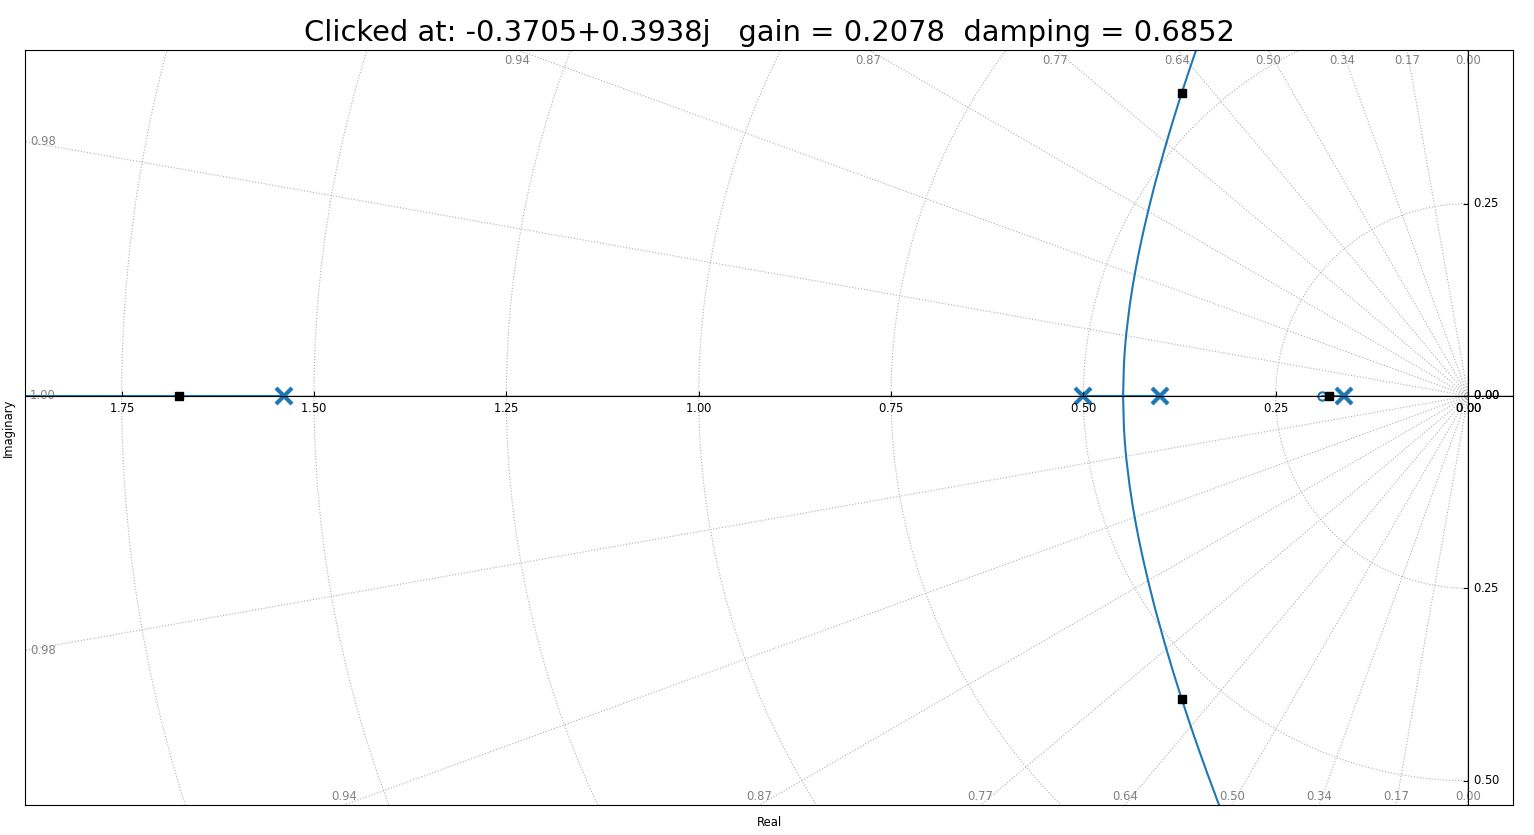
\includegraphics[width=0.9\textwidth]{Images/PD_compensated_root_locus.jpg}
    \caption{Quỹ tích nghiệm của hệ thống bù PD}
\end{figure}
\noindent Đối với phần tích phân ID, hệ thống giả định sử dụng $G_c(s) = \frac{s+0.01}{s}$. Khi đó, hàm truyền tổng hợp PID là:
$$G_{\text{PID}}(s) = K \cdot \frac{(s+z_c)(s+z_{PI})}{s} = \frac{0.5857(s+0.19)(s+0.01)}{s}$$
Kiểm tra quỹ tích nghiệm cho thấy bộ điều khiển PID đã đạt yêu cầu thiết kế với Peak Time $T_p = 8 \text{ s}$ và Overshoot $\%OS = 5\%$.
\begin{figure}[H]
    \centering
    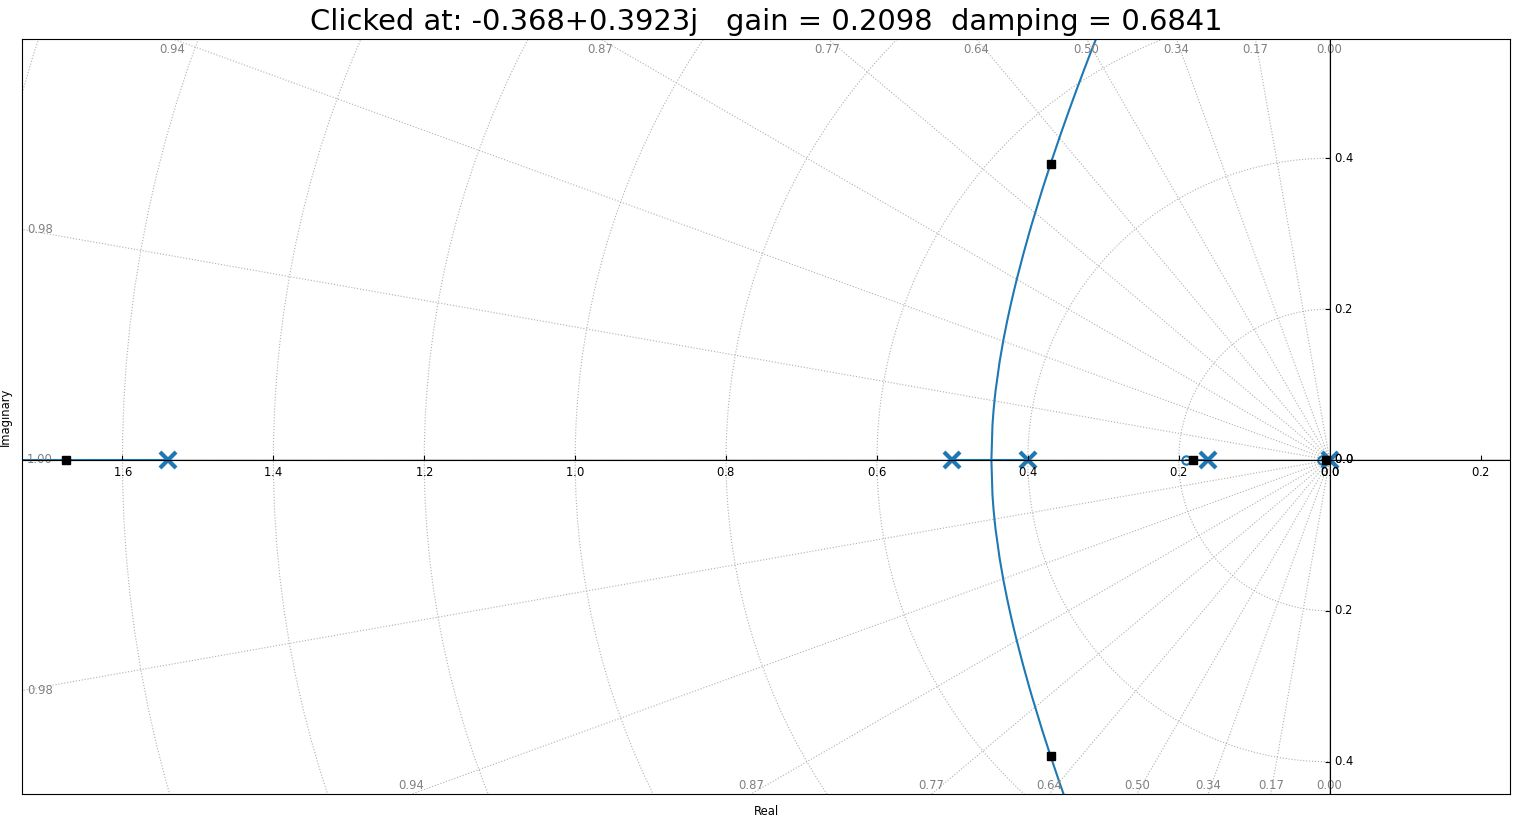
\includegraphics[width=0.9\textwidth]{Images/PID_compensated_root_locus.jpg}
    \caption{Quỹ tích nghiệm của hệ thống bù PID}
\end{figure}
\section{Số hóa hàm truyền hệ thống}
Sau khi có bộ PID, hệ thống hiện tại đang như sau:
\begin{figure}[H]
    \centering
    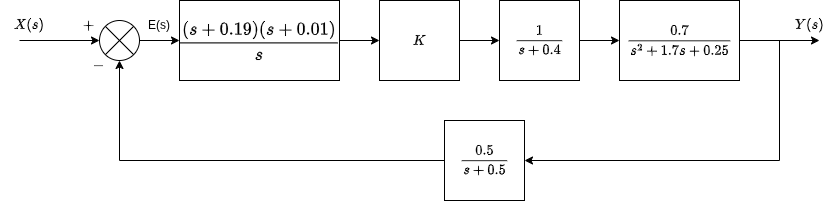
\includegraphics[width=0.9\textwidth]{Images/PID_system.png}
    \caption{Hệ thống sau khi có bộ điều khiển PID}
\end{figure}
Từ đây, ta tìm được hàm truyền vòng kín của hệ thống là:
$$ T(s) = \frac{G(s)}{1 + G(s)H(s)} $$
$$ T(s) = \frac{\frac{(s+0.19)(s+0.01)}{s} \cdot K \cdot \frac{1}{s + 0.4} \cdot \frac{0.7}{s^2+1.7s+0.25}}{1 + \frac{(s+0.19)(s+0.01)}{s} \cdot K \cdot \frac{1}{s + 0.4} \cdot \frac{0.7}{s^2+1.7s+0.25} \cdot \frac{0.5}{s + 0.5}} $$
$$T(s) = \frac{1.1714s^3 + 0.81998s^2 + 0.12182s + 0.00111}{s^5 + 2.6s^4 + 2.5657s^3 + 0.68214s^2 + 0.05111s + 0.00111}$$

Để số hóa được hàm truyền, ta sử dụng phương pháp Tustin:
$$ T(z) = T(s)|_{s = \frac{2}{T_s} \frac{z - 1}{z + 1}}$$

\section{Mô phỏng và đánh giá}
Sau khi có hàm truyền $T(z)$, ta tìm đáp ứng nhảy bậc của nó. Kết quả của đáp ứng được thể hiện dưới đây:
\begin{figure}[H]
    \centering
    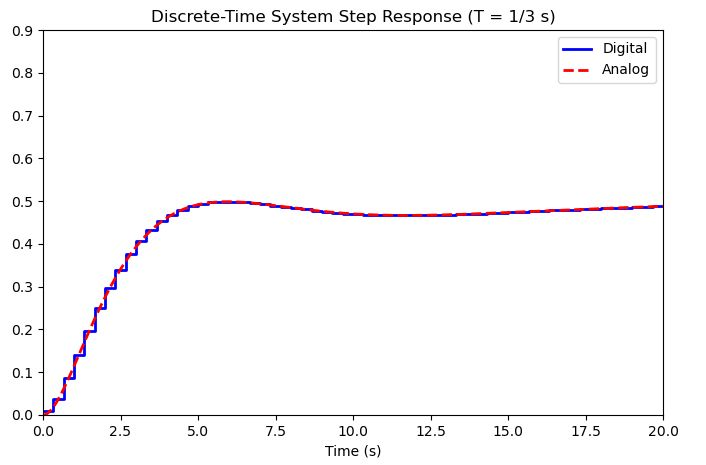
\includegraphics[width=0.9\textwidth]{Images/simulation_result.jpg}
    \caption{Kết quả mô phỏng đáp ứng hệ thống}
\end{figure}
Về đánh giá kết quả:
\begin{enumerate}
    \item Overshoot $\%OS$ 
    Giá trị này có thể được kiểm tra $$\%OS = \frac{Peak - Steady}{Steady} \times 100\% = \frac{0.5 - 0.48}{0.48} \times 100\% \approx 6\%$$
    Điều này cho thấy hệ thống có đạt yêu cầu Overshoot.

    \item Peak Time $T_p$
    Peak Time của hệ thống theo mô phỏng ở khoảng 5.3 s, nhanh hơn so với yêu cầu bài toán.

    \item Zero Steady State
    Trong đồ thị, hệ thống ổn định từ giây thứ 10 trở đi. Kết quả đúng với yêu cầu đề bài.
\end{enumerate}
\end{document}